\documentclass{article}
\usepackage[utf8]{inputenc}
\usepackage{graphicx} % For images

\title{Report DM project}
\author{Alessio Russo, Michele Zoncheddu}
\date{October 2020}

\begin{document}

\maketitle

\tableofcontents

\section{Introduction}
The aim of the report is to describe the customer profile and his purchasing behavior by analyzing a given dataset, \textit{supermarket.csv},  following the \textit{KDD} process. 
Each entry in the dataset represent a single item bought by a costumer in a given shopping session. An entry is composed by 8 attributes that contains information about the shopping session, date, customer and about the product bought.

The analysis is composed in 3 main phases:
\begin{itemize}
    \item Data Understanding
    \item Data Preparation
    \item Clustering
\end{itemize}

\section{Data Understanding}
The dataset is a matrix composed by 471910 rows and 8 columns. Each row gives information about a single purchase of a product during a shopping session of a given customer.

\subsection{Data type, semantic and quality}
In this section is illustrated the type and the semantic of each attribute. 
\subsubsection{BasketID}
\begin{itemize}
    \item type: nominal/categorical;
    \item semantic: it describes the shopping session. A group of entries with the same BasketID belongs to the same shopping session. There are 3 types of BasketID and we assume that the ones starting with letter `A' are aborted transactions and the ones starting with letter `C' are canceled transaction. If one entry has BasketID starting with `A' or `C', all the others  with the same BasketID start with `A' or `C';
    \item quality: there are no missing values.
\end{itemize}

\subsubsection{BasketDate}
\begin{itemize}
    \item type: interval attributes;
    \item semantic: it describes the date of the purchase in the format \textit{yyyy-mm-dd hh-mm}. The analyzed time interval is between 2010-12-01 and 2011-12-09;
    \item quality: there are no missing values.
\end{itemize}

\subsubsection{Sale}
\begin{itemize}
    \item type: numerical ratio;
    \item semantic: it describes the unitary price of the product bought by the customer in a single shopping session;
    \item quality: by using statistical analysis and visualization techniques, we noted that there some negative and huge amount of sales w.r.t the mean. The negative sale is related to the BasketID that have a leading `A' and so, as mentioned before, we consider them “aborted transaction". There are no missing values.
\end{itemize}
\begin{center}
	\begin{figure}[ht!]
		\makebox[\textwidth]{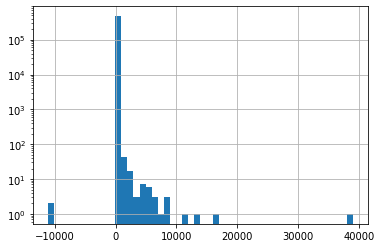
\includegraphics[width=0.35\paperwidth]{img/sale.png}}
		\caption{Sale distribution.}
	\end{figure}
\end{center}

\subsubsection{CustomerID}
\begin{itemize}
    \item type: nominal/categorical; 
    \item semantic: it uniquely identify the customer during its shopping sessions;
    \item quality: 13\% of CustomerIDs are missing. Given the high number of $null$ CustomerIDs, we decided to consider them valid, under certain conditions (see sect).
\end{itemize}

\subsubsection{CustomerCountry}
\begin{itemize}
    \item type: nominal/categorical;
    \item semantic: it represents the nationality of the customer;
    \item quality: there are no missing values, but 340 records have “Unspecified" as country. The remaining 37 values are all real countries.
\end{itemize}

\begin{center}
	\begin{figure}[ht!]
		\makebox[\textwidth]{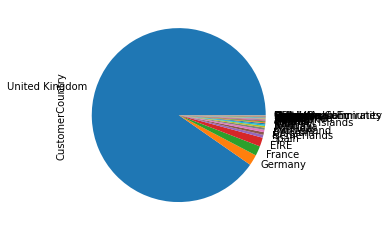
\includegraphics[width=0.4\paperwidth]{img/countries.png}}
		\caption{Customer countries distribution.}
	\end{figure}
\end{center}

\subsubsection{ProdID}
\begin{itemize}
    \item type: nominal/categorical;
    \item semantic: it uniquely identifies the product bought by a customer;
    \item quality: after a deeper analysis we've detected some unusual and erroneous ProdIDs in terms of length and meaning, such as “M", “POST" or “CRUK" (Charitable organization).
\end{itemize}

\subsubsection{ProdDescr}
\begin{itemize}
    \item type: categorical;
    \item semantic: it's the product name;
    \item quality: 0.15\% of the descriptions are missing. Among the present ones, we found some unusual and erroneous descriptions, such as “POSTAGE" or “OOPS ! adjustment".
\end{itemize}
\begin{center}
	\begin{figure}[ht!]
		\makebox[\textwidth]{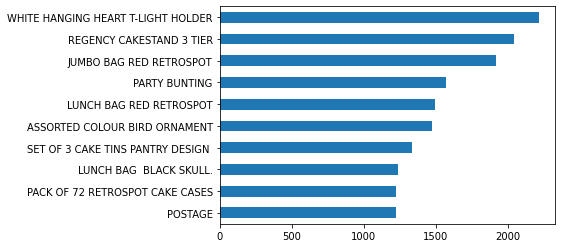
\includegraphics[width=0.5\paperwidth]{img/top10prod.png}}
		\caption{Top 10 products.}
	\end{figure}
\end{center}

\subsubsection{Qta}
\begin{itemize}
    \item type: numerical ratio;
    \item semantic: it represents the quantity of products per transaction;
    \item quality: by using statistical analysis and visualization techniques, we noted that there some negative and huge amount of quantities w.r.t the mean. All the records with negative quantities have BaskedIDs with a leading `C', that we assume means "canceled order". There are no missing values.
\end{itemize}

\begin{center}
	\begin{figure}[ht!]
		\makebox[\textwidth]{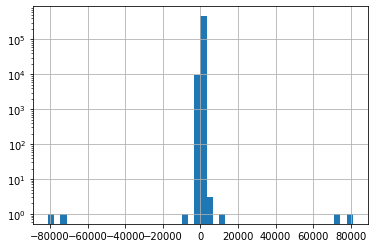
\includegraphics[width=0.30\paperwidth]{img/qta.png}}
		\caption{Quantity distribution.}
	\end{figure}
\end{center}


\section{Data Preparation}

\end{document}
